\documentclass[tikz, border=2mm]{standalone}
\usepackage{tikz}
\usepackage{xcolor}
\usetikzlibrary{shapes, arrows.meta, positioning, backgrounds, calc, fit}

\definecolor{rwthblue}{HTML}{00549f}
\definecolor{rwthmediumblue}{HTML}{407FB7}
\definecolor{rwthlightblue}{HTML}{e8f1fa}
\definecolor{rwthlightblue}{HTML}{8EBAE5}
\definecolor{rwthverylightblue}{HTML}{C7DDF2}
\definecolor{rwthgreen}{HTML}{57AB27}
\definecolor{rwthlightgreen}{HTML}{8DC060}

\begin{document}

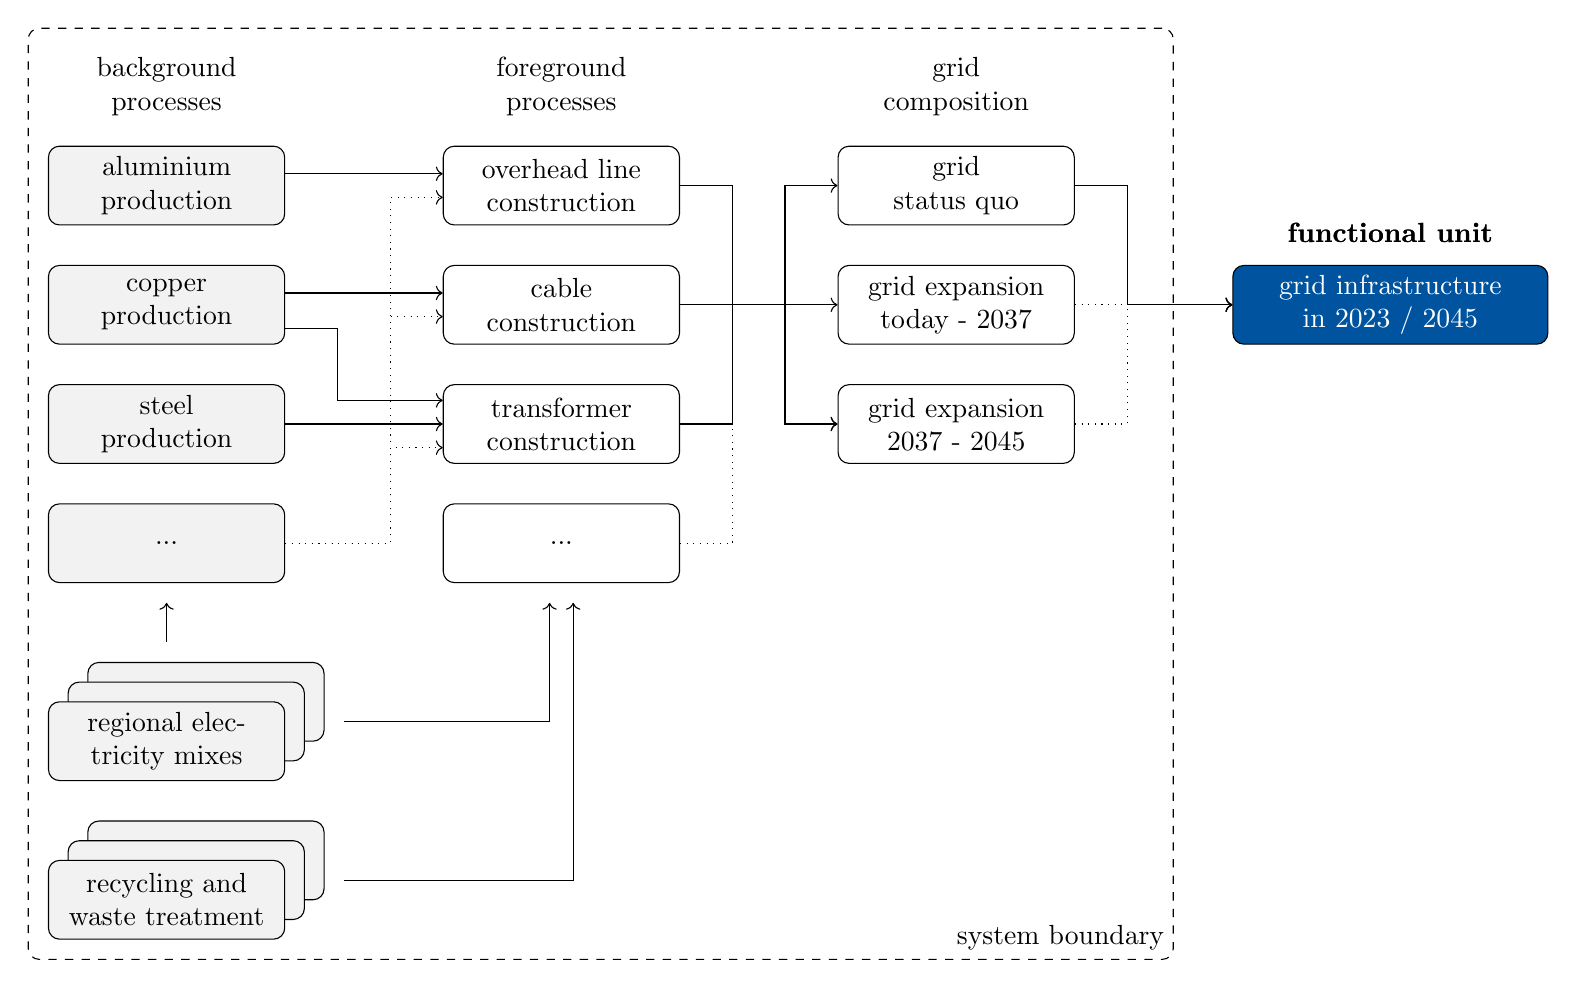
\begin{tikzpicture}[node distance=0.5cm and 2cm,
                    auto, 
                    background_process/.style={rectangle, draw, align=center, rounded corners, minimum height=1cm, minimum width=3cm, fill=gray!10},
                    foreground_process/.style={rectangle, draw, align=center, rounded corners, minimum height=1cm, minimum width=3cm},
                    expansion_period/.style={rectangle, draw, align=center, rounded corners, minimum height=1cm, minimum width=3cm},
                    functional_unit/.style={rectangle, draw, align=center, rounded corners, minimum height=1cm, minimum width=4cm, fill=rwthblue, text=white},
                    ]

    % Background processes
    \node[background_process] (aluminium) {aluminium\\production};
    \node[background_process, below=of aluminium] (copper) {copper\\production};
    \node[background_process, below=of copper] (steel) {steel\\production};
    \node[background_process, below=of steel] (further_processes) {...};
    \node[background_process, below=of further_processes, yshift=-0.5cm, xshift=0.5cm] (electricity3) {};
    \node[background_process, below=of further_processes, yshift=-0.75cm, xshift=0.25cm] (electricity2) {};
    \node[background_process, below=of further_processes, yshift=-1cm] (electricity1) {regional elec-\\tricity mixes};
    \node[background_process, below=of electricity1, yshift=-0cm, xshift=0.5cm] (waste3) {};
    \node[background_process, below=of electricity1, yshift=-0.25cm, xshift=0.25cm] (waste2) {};
    \node[background_process, below=of electricity1, yshift=-0.5cm] (waste1) {recycling and\\waste treatment};
    
    \node[align=center] (background_processes) at ($(aluminium.north) + (0,0.75cm)$) {background\\processes};

    % Foreground processes
    \node[foreground_process, right=of aluminium] (line) {overhead line\\construction};
    \node[foreground_process, right=of copper] (cable) {cable\\construction};
    \node[foreground_process, right=of steel] (transformer) {transformer\\construction};
    \node[foreground_process, right=of further_processes] (further_components) {...};
    \node[align=center] (foreground_processes) at ($(line.north) + (0,0.75cm)$) {foreground\\processes};
    
    % Expansion scenarios
    \node[expansion_period, right=of line] (statusquo) {grid\\status quo};
    \node[expansion_period, below=of statusquo] (expansion2037) {grid expansion\\today - 2037};
    \node[expansion_period, below=of expansion2037] (expansion2045) {grid expansion\\2037 - 2045};
    \node[align=center] (grid_amounts) at ($(statusquo.north) + (0,0.75cm)$) {grid\\composition};

    % Functional Unit
    \node[functional_unit, right=of expansion2037] (fu) {grid infrastructure\\ in 2023 / 2045};
    \node[align=center] (fu_text) at ($(fu.north) + (0,0.4cm)$) {\textbf{functional unit}};

    % System boundary
    \node[align=center] (system_boundary) at ($(fu.north) + (0,0.4cm)$) {\textbf{functional unit}};
    
    % Large rectangle around everything except functional unit and scenario
    \begin{scope}[on background layer]
        \node[draw, rounded corners, dashed, fit=(background_processes) (foreground_processes) (aluminium) (copper) (steel) (further_processes) (electricity3) (electricity2) (electricity1) (waste3) (waste2) (waste1) (line) (cable) (transformer) (further_components) (statusquo) (expansion2037) (expansion2045), inner ysep = 0.25cm, inner xsep=0.75cm, xshift = 0.5cm, label={[anchor=south east]south east:system boundary}] {};
    \end{scope}
    
    % Materials to components
    \draw[->] ($(aluminium.east) + (0, 0.15cm)$) -- ($(line.west) + (0, 0.15cm)$);
    \draw[->] ($(copper.east) + (0, 0.15cm)$) -- ($(cable.west) + (0, 0.15cm)$);
    \draw[->] ($(copper.east) + (0, -0.3)$) -| ($(copper.east)!.333!(transformer.west)$) |- ($(transformer.west) + (0, 0.3cm)$);
    \draw[->] (steel) -- (transformer);
    
    % Further component inputs "..."
    \draw[->, dotted] (further_processes.east) -| ($(further_processes.east)!.666!(line.west)$) |- ($(line.west) + (0, -0.15cm)$);
    \draw[->, dotted] (further_processes.east) -| ($(further_processes.east)!.666!(cable.west)$) |- ($(cable.west) + (0, -0.15cm)$);
    \draw[->, dotted] (further_processes.east) -| ($(further_processes.east)!.666!(transformer.west)$) |- ($(transformer.west) + (0, -0.3cm)$);
    
    % Electricity mixes
    \draw[->] ($(electricity3.north) + (-0.5cm,0.25cm)$) -- ($(further_processes.south) + (0,-0.25cm)$);
    \draw[->] ($(electricity2.east) + (0.5cm,0)$) -| ($(further_components.south) + (-0.15,-0.25cm)$);

    % waste
    \draw[->] ($(waste2.east) + (0.5cm,0)$) -| ($(further_components.south) + (0.15,-0.25cm)$);

    % Components to expansion periods
    \draw[->] (cable) -- (expansion2037);
    \draw[->] (line.east) -| ($(cable.east) + (0.666cm,0)$) -- ($(cable.east) + (1.333cm,0)$) |- (statusquo.west);
    \draw[->] (transformer.east) -| ($(cable.east) + (0.666cm,0)$) -- ($(cable.east) + (1.333cm,0)$) |- (expansion2045.west);
    \draw[->, dotted] (further_components) -| ($(cable.east) + (0.666cm,0)$) -- ($(cable.east) + (1.333cm,0)$) |- (expansion2045.west);

    % Expanison periods to FU
    \draw[->] ($(statusquo.east)$) -| ($(statusquo.east)!.333!(fu.west)$) |-  (fu);
    \draw[->, dotted] (expansion2037) -- (fu);
    \draw[->, dotted] ($(expansion2045.east)$) -| ($(expansion2045.east)!.333!(fu.west)$) |-  (fu);

\end{tikzpicture}

\end{document}
